\documentclass[tikz]{standalone}
% Preamble
	\usepackage{fullpage} % Package to use full page
	\usepackage{parskip} % Package to tweak paragraph skipping
	\usepackage{tikz} % Package for drawing
	\usepackage{amsmath}
	\usepackage{hyperref}
	\usepackage{amsmath,amssymb}
	\usepackage{color}
	\usepackage[version=4]{mhchem} 
	\usepackage{bm}
	\usepackage{verbatim}
	\usepackage{tkz-euclide}
    \usetkzobj{all}
	
	
	\usetikzlibrary{arrows,automata,positioning,backgrounds,calc,fadings}
	\usetikzlibrary{decorations.shapes}
	\usetikzlibrary{shapes,arrows,automata,positioning,fit,backgrounds,petri}
	\usetikzlibrary{fadings,decorations.pathmorphing}
	\usetikzlibrary{arrows,shapes}
	
% Define different styles:
    %-------------
    % Blue colors
        \definecolor{deepskyblue}{cmyk}{1,0.25,0.0,0}
        \definecolor{picassoblue}{cmyk}{0.99,0.53,0.0,0.1}
    % Green colors
        \definecolor{springgreen}{cmyk}{1,0,0.8,0}
    % Yellow colors
        \definecolor{gold7}{cmyk}{0,0.33,1,0}
    % Orange colors
        \definecolor{burntorange}{cmyk}{0,0.52,1,0}
    %-------------
        \tikzstyle{blue} = [circle,thick,inner color = picassoblue!100, outer color = deepskyblue!80, opacity = 0.9]
        \tikzstyle{vertex}=[rectangle,fill=white,minimum size=10pt,inner sep=0pt]
    %-------------					
\begin{document}
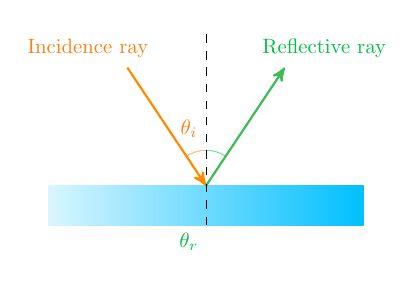
\begin{tikzpicture}[>=stealth',shorten >=0pt,auto,node distance=3cm]
%-------------------------start grid code ---------------------
	%\def\figWd{4.5};
    %\def\figHt{4.5};
					
	%\draw[step=0.5,very thin, black!15] (-0.5,-0.5) grid (\figWd,\figHt);
	%\draw[thick,->] (0,0) -- (\figWd,0) node[anchor=north west] {$x$};
    %\draw[thick,->] (0,0) -- (0,\figHt) node[anchor=south east] {$y$};
					
	%\foreach \x in {0,...,\figWd} 
	%\draw (\x cm,1pt) -- (\x cm,-1pt) node[anchor=north] {$\x$};
	%\foreach \y in {0,...,\figHt}
    %\draw (1pt,\y cm) -- (-1pt,\y cm) node[anchor=east] {$\y$};
%--------------------------end grid code ----------------------
%--------------------start object code --------------------
	\coordinate (surfaceSW) at (0,0.5);
	\coordinate (surfaceNE) at (4,1);
	
	\filldraw[draw=none, left color = white!85!deepskyblue, right color = deepskyblue] (surfaceSW) rectangle (surfaceNE);
	
	\coordinate (perpstart) at (2,0.5);
	\coordinate (perpend) at (2,3);
	
	%Incidence Ray
	\coordinate (istart) at (1,2.5);
	\coordinate (iend) at (2,1);
	\tkzMarkAngle[draw=burntorange,fill=orange!80,opacity=.5,size=.45](perpend,iend,istart)
	\tkzLabelAngle[vertex,scale=0.75](perpend,iend,istart){\textcolor{burntorange}{$\theta_i$}}
	\path[->,orange!90!yellow,thick] (istart) edge [bend left=0] node{} (iend);
	
	\coordinate (ilabel) at (0.5,2.75);
	\node[vertex,scale=0.75] (ilabel) at (ilabel) {\textcolor{burntorange}{Incidence ray}};
	
	%Refractive Ray
	\coordinate (rstart) at (2,1);
	\coordinate (rend) at (3,2.5);
	\tkzMarkAngle[draw=green!75!blue,fill=springgreen!80,opacity=.5,size=.45](rend,rstart,perpend)
	\tkzLabelAngle[vertex,scale=0.75](perpend,rstart,rend){\textcolor{green!75!blue}{$\theta_r$}}
	\path[->][springgreen!75!yellow,thick] (rstart) edge [bend left=0] node{} (rend);
	
	\coordinate (jlabel) at (3.5,2.75);
	\node[vertex,scale=0.75] (jlabel) at (jlabel) {\textcolor{green!75!blue}{Reflective ray}};
	
	%Perpendicular line
	\path[black,dashed] (perpstart) edge [bend left=0] node{} (perpend);
%-------------------------end object code-----------------------
\end{tikzpicture}
\end{document}
				